\section{色域最大化 -- 第四个基色}
从前面的色品图中我们可以看到RGB三色光所租成的色域,很明显的是,在此基础上再加上一个合适的单色光,必定会有更大的色域,由于时间不够,本文只对llab的数据进行探究,采用蓝色的光谱进行``位移'',视为新的单色光。本节以CIE 1931-XYZ色品图与色彩匹配函数作为探究前提。

\subsection{预搜寻--人工感知}

首先我们对色域三角形的三条边进行延拓,如图\ref{fig:sd1931-LINE}所示。

\begin{figure}[htbp]
    \centering
    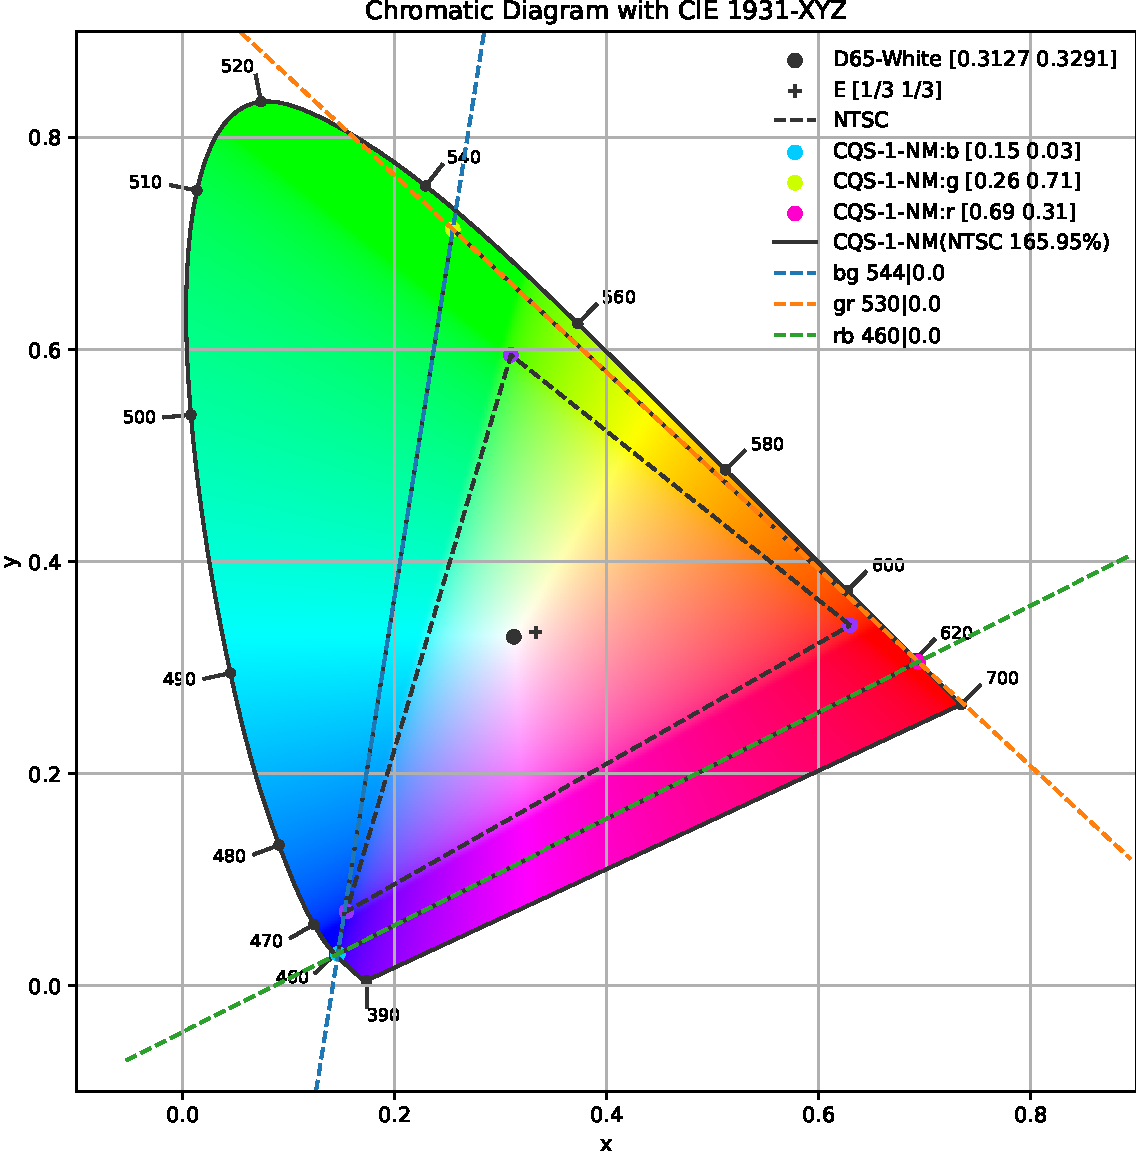
\includegraphics[width=0.65\textwidth]{./imgs/sec5/CQS-1-NM-1931-Line.pdf}
    \caption{CIE 1931-XYZ色彩匹配函数下LED色域三角形延展}
    \label{fig:sd1931-LINE}
\end{figure}

从图上我们可以看到,左侧的空隙较大,若讨论单色光必定在460nm至530nm之间的单色光。即便讨论的不是单色光,直觉上第四个光源要使得色域最大化,应该要在蓝绿色分界线上,比如说靠近500$\sim$510nm的单色光的光谱直觉上会得到最大的色域。做研究不能只靠直觉,还得拥有数据,因此我们将在下一小节``复制平移''一个蓝色光源视为``第四色'',探究最大色域范围。

\subsection{程序搜寻--计算面积}

本小节的下的蓝光的中心波长为457nm,两个半功率点分别位于为451nm与463nm,因此我们最大蓝移为451nm$\rightarrow$380nm,最大红移为463nm$\rightarrow$780nm。蓝移部分有71个点,红移部分有317个点,将这些点绘制到色品图上,如图\ref{fig:sd1931-BLUEMOVE}所示。

\begin{figure}[htbp]
    \centering
    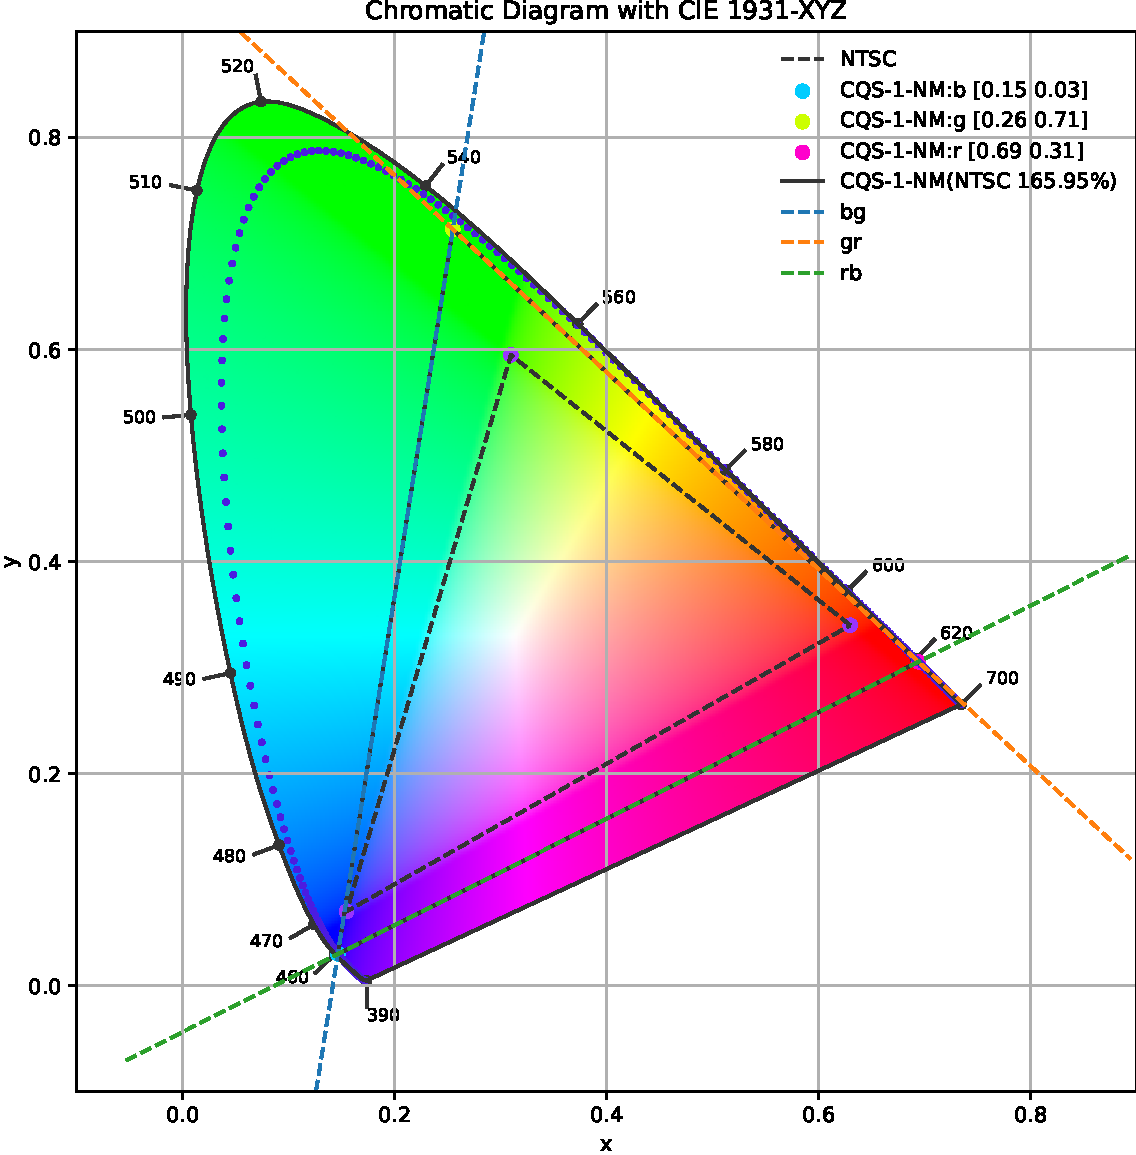
\includegraphics[width=0.65\textwidth]{./imgs/sec5/CQS-1-NM-4.pdf}
    \caption{蓝色LED平移}
    \label{fig:sd1931-BLUEMOVE}
\end{figure}

从图上我们可以得知,由于llab的LED数据较为纯净,平移后的结果比较靠近纯色光,在蓝移区基本贴近(需要放大看,这幅图有点吵眼睛)纯色光组成的马蹄边界。红移区需要到560nm后才基本贴近。由于第四个色出现的位置和面积计算有一些关联,比如说530nm$\sim$544nm的线段,若第四个色取自于这里,则得忽略绿色,进行新三角形的计算,而红色处在gr和rb交界上,蓝色也在bg和rb交界上,则可忽略这个问题,除了上面说的绿色特殊位置,都可以认为是一个四边形的计算,这些四边形和三角形的计算都可以由鞋带公式解决,以下部分操作部分由人工设置,非完全自适应。后续操作流程如下所示。
\begin{itemize}
    \item [1. ]计算特殊区域三角区,得到该三角区范围为534$\sim$542nm(平移后的中心),详细请见{\bf scripts/plot\_sd4\_findP.py}文件。
    \item [2. ]根据区域分段计算面积(采用鞋带公式计算三角形与四边形的面积),然后保存在一个数组中
    \item [3. ]寻找这个数组中的最大元素,找到对应的xy
    \item [4. ]根据xy值转到xyY系统再转XYZ系统再转sRGB得到对应颜色
    \item [5. ]画出该光功率谱,并查阅相关资料获取该RGB值的颜色名称
\end{itemize}
以上计算的完成为穷尽法,详情请见文件{\bf scripts/plot\_sd4\_final.py}。我们发现,红移51nm后得到以508nm为中心的光的面积最大,为0.24164,RGB值为\#00FF6B(归入0$\sim$255后取四舍五入),即$(r,g,b)=(0,255,107)$也符合我们前面的直觉。该颜色的光谱图\ref{fig:spd1931-color4}如所示。

\begin{figure}[htbp]
    \centering
    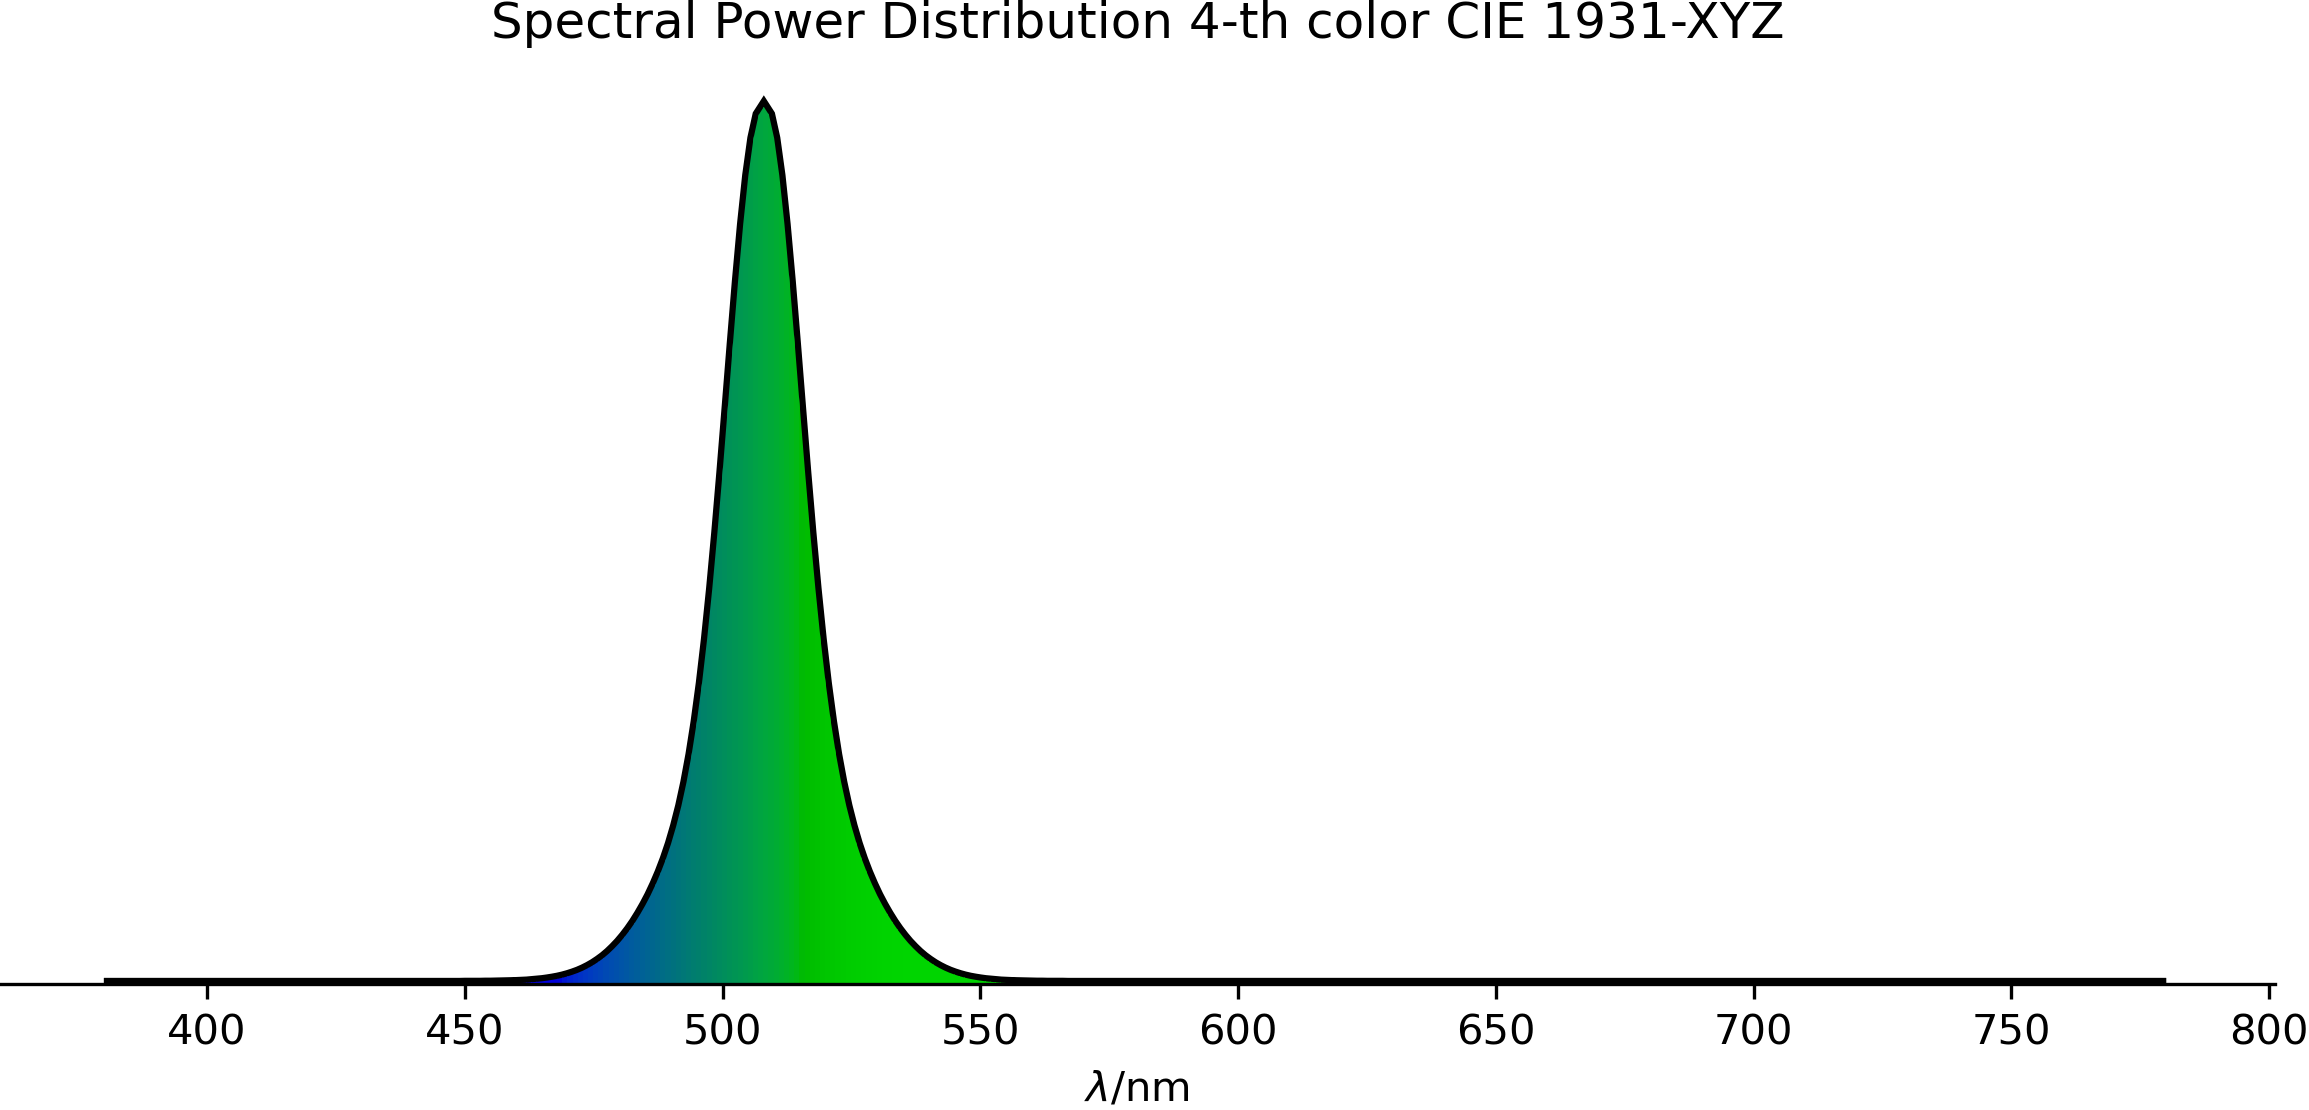
\includegraphics[width=0.65\textwidth]{./imgs/sec5/CQS-1-NM-spd-4.png}
    \caption{第四光源的光谱图(CIE 1931-XYZ)}
    \label{fig:spd1931-color4}
\end{figure}


处理后得到的最大面积色域与色品图如图所示\ref{fig:spd1931-4final}所示。

\begin{figure}[htbp]
    \centering
    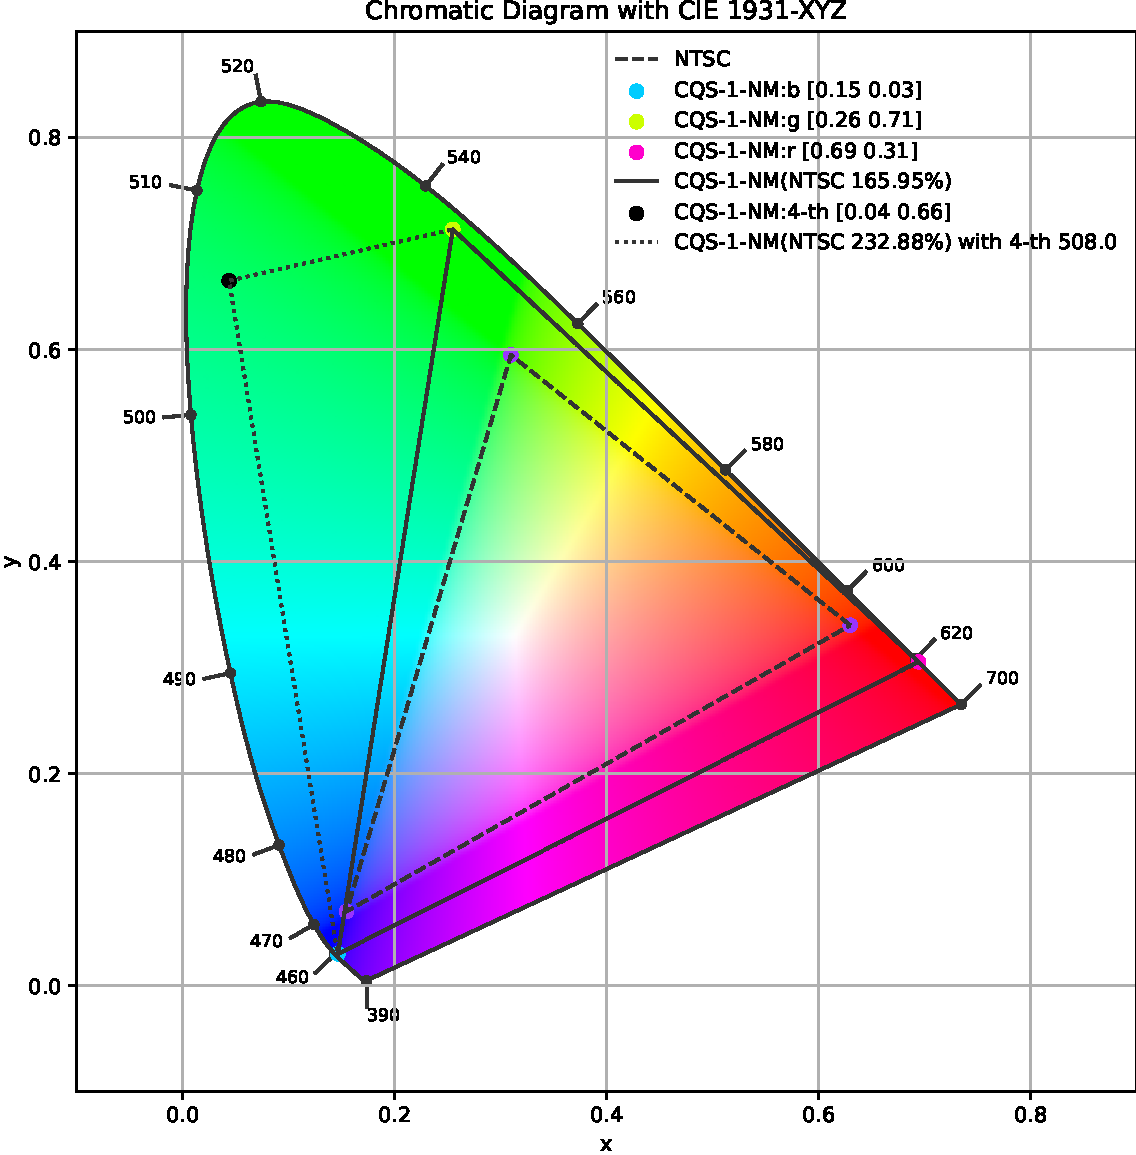
\includegraphics[width=0.65\textwidth]{./imgs/sec5/CQS-1-NM-4-final.pdf}
    \caption{第四光源的光谱图(CIE 1931-XYZ)}
    \label{fig:spd1931-4final}
\end{figure}

\subsection{结论}
我们从上面了解到该颜色光的RGB为$(r,g,b)=(0,255,107)$,换为16进制为\#00FF6B,这种颜色的名字没有确切定义\footnote{https://www.htmlcsscolor.com/hex/00FF6B},类似于春绿色(Spring Green,\#00FF7F),本文暂称其为类春绿色。我们认为加上类春绿色的光源将会令llab数据的色域范围最大。由于时间问题,本文不讨论P2226与P3030的情况。由于该部分完成的较为急迫,代码相对繁杂且冗余过多。

